\subsection{Product perspective}
\subsubsection{Scenarios}

\begin{enumerate}
   \item \textbf{Creating a Tournament:} \\
    John, a university professor, wants to give his students the opportunity to improve their skills before the upcoming exam session. To achieve this, he logs into the CKB platform using his educator account. Once logged in, John initiates the process by creating a new tournament.
    During the tournament creation, John writes a comprehensive description of the game. Following the tournament's creation, the CKB platform notifies all subscribed students about the newly initiated competition.
   
%       \begin{itemize}
%            \item Educator logs in to the CKB platform;
%            \item Educator creates a new tournament;
%            \item Educator sets tournament details, including a description, start and end dates, and any specific rules;
%            \item CKB notifies all subscribed students about the new tournament.
%        \end{itemize}

   \item \textbf{Creating a Code Kata Battle:} \\
Sophia, to contribute to her colleague Liam's programming tournament, takes the initiative to create a new Code Kata Battle within the existing tournament. Liam has granted her the authorization to add Code Kata Battles to this specific tournament.
Sophia begins by logging into the CKB platform (with her educator account) and navigating to Liam's tournament section. Here, she uploads the challenge details, composing a descriptive introduction to the Code Kata and including the necessary software project files along with building automation scripts to facilitate a seamless development and evaluation process. Moving forward, Sophia configures the battle parameters, specifying the minimum and maximum number of students permitted per group. She sets a registration deadline, indicating when students should form or join teams for the battle, and a final submission deadline. Additionally, she customizes scoring configurations to tailor the evaluation process for this specific challenge.
Upon successfully creating the Code Kata Battle, the CKB platform notifies all subscribed students within Liam's tournament. Students receive notifications about the newly introduced challenge, including essential details such as registration and submission deadlines.
 
%\begin{itemize}
%            \item Educator selects a tournament to create a code kata battle within;
%            \item Educator uploads the code kata, including the description, software project, and build automation scripts;
%            \item Educator sets the minimum and maximum number of students per group, registration deadline, final submission deadline, and additional scoring configurations;
%           \item CKB platform notifies all subscribed students about the new battle.
%      \end{itemize}

    \item \textbf{Student partecipates to a Battle:} \\
    Olivia, willing to play a C++ coding challenge with her coding club friends, initiates her participation by logging into the CKB platform. Within the platform, she navigates to the desired tournament and selects the specific battle she wishes to join. Once Olivia joins the battle, she enters the subscription phase.
During the subscription phase, Olivia invites her friends to form a team, ensuring to respect the specified minimum and maximum number of members for that particular battle. Her friends, upon receiving the invitation, log into the CKB platform and promptly accept her invitation to become members of the team.
To submit their code, Olivia and her teammates fork the designated GitHub repository, and they set up an automated workflow using GitHub Actions to streamline the continuous integration process. The team can submit their code by committing changes to the main branch.
The CKB platform is triggered on each push, pulling the latest sources and executing the necessary tests to calculate and promptly update the team's score. This real-time scoring mechanism ensures that students and educators have instantaneous access to the latest results, fostering an environment of transparency and healthy competition.

\comment{TEAM NON ACCETTATO? ISCRIZIONI?}
    
%        \begin{itemize}
 %           \item Students log in to the CKB platform;
  %          \item Students join a code kata battle individually or invite others to form a team;
   %         \item Students adhere to the minimum and maximum number of students per group set for the battle.
    %        \item Students fork the GitHub repository and set up automated workflows using GitHub Actions;
     %       \item Students commit code changes to the main branch;
            %\item CKB platform is triggered on each push, pulling the latest sources and running tests to calculate and update the team's score.
            %\item Scores are updated in real-time on the platform, visible to both students and educators.
%        \end{itemize}

    \item \textbf{Educator manually evaluates Students' solutions:} \\
    As the submission deadline for Jacob's battle approaches the consolidation phase begins. Once the deadline expires, the CKB platform automatically evaluates essential components such as functional aspects, timeliness, and source code quality. This automated evaluation ensures a comprehensive and standardized assessment of each participating group's performance. In addition to the automated evaluation, Jacob, as the organizer, takes an extra step to guarantee the fairness of the competition. He personally reviews and evaluates the submissions from all participating groups, applying his expertise to acknowledge exceptional efforts and contributions. The final scores are finally assigned, marking the conclusion of the consolidation phase. At this point, all scores become visible to the users. 
    
%        \begin{itemize}
%            \item After the submission deadline, there is a consolidation stage;
%            \item CKB platform automatically evaluates functional aspects, timeliness, and source code quality;
%            \item Educator may manually evaluate and assign a personal score;
%            \item If manual evaluation is required, the educator reviews and scores the sources produced by each team;
%        \end{itemize}

    \item \textbf{Tournament Closure and Notifications:} \\
    Emily decides to conclude her tournament on the CKB platform. Following this decision, the CKB platform promptly took action, notifying all students who actively participated in the tournament about its closure. Simultaneously, the platform updates the personal tournament scores for each student involved. This ensures that participants are promptly informed of their final standings and achievements in the context of the concluded tournament.
    
%        \begin{itemize}
%            \item Educator closes the tournament;
%            \item CKB platform notifies all students involved in the tournament;
%            \item Personal tournament scores are updated for each student.
%        \end{itemize}

    \item \textbf{Gamification Badges:}
    Robert has recently created a tournament and wants to improve the gamification aspect of the competition by introducing badges. To integrate these badges into the  CKB platform, Robert utilizes the platform's commands, specifying distinct titles and rules for each badge. Students earn badges based on their performance in battles. After each battle, the CKB platform automatically assesses and assigns badges to students who have fulfilled the specified requirements for each badge.
The badges, complete with their titles and associated rules, are displayed for all participants.
    
%        \begin{itemize}
%            \item Educator creates gamification badges for the tournament;
%            \item Badges have titles and rules based on predefined variables;
%            \item Students earn badges based on their performance in battles.
%            \item Badges are displayed with their titles and associated rules;
%        \end{itemize}
    
\end{enumerate}

\subsubsection{Domain class diagram}
\comment{Descrizione del class diagram}

\begin{figure}[h!]
  \centering
  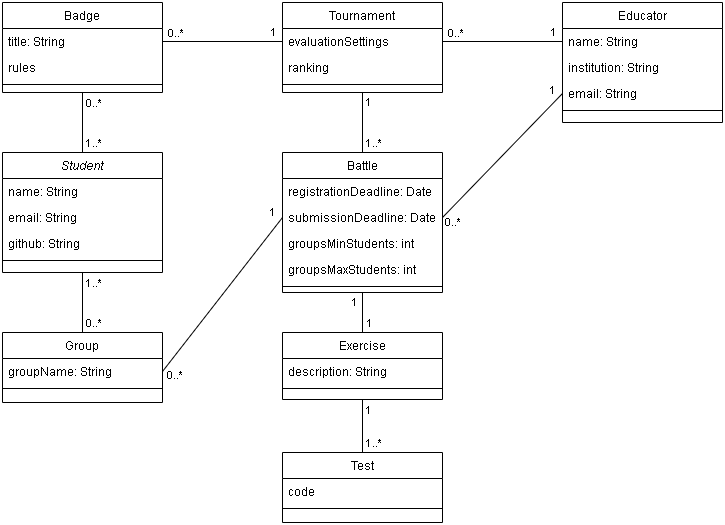
\includegraphics[width=0.8\textwidth]{Images/ClassDiagramRASD.png}
  \caption{Domain class diagram}
  \label{fig:ClassDiagram}
\end{figure}

\subsubsection{Statecharts}

%\comment{Fare i diagrammi ed introduzione: plantuml + plantext}

The CKB platform involves several key states and transitions to facilitate the seamless execution of code kata battles and tournaments. The primary states and transitions are described below:

\begin{enumerate}
    
    \item \textbf{Tournament Lifecycle:} \\
    Upon the creation of a tournament, the Registration state commences, enabling students to submit their applications. Upon the conclusion of the registration phase, the tournament seamlessly transitions to the Started state, officially allowing users to subscribe to the battles. Upon reaching its conclusion, the educator who initiated the tournament holds the authority to close it, guiding it into the Closed state. This state transition mechanism ensures a structured progression throughout the tournament lifecycle.
    
    \begin{figure}[h!]
          \centering
          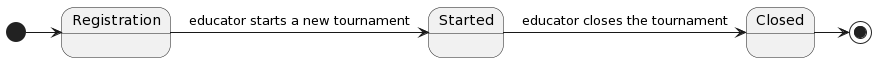
\includegraphics[width=1\textwidth]{Images/TournamentLifecycle.png}
          \caption{Tournament Lifecycle}
          \label{fig:TournamentLifecycle}
    \end{figure}

    \item \textbf{Code Kata Battle Lifecycle:} \\
    Upon the creation of a code kata battle, it assumes the RegistrationOpen state, enabling students to participate by entering the battle and forming teams. Following the expiration of the registration deadline, the state seamlessly transitions to Started, marking the commencement of the game.

Upon reaching its conclusion, the battle undergoes a state transition. If necessary, and at the discretion of the educator, it can move to the Consolidation state for a manual review of the code. Alternatively, if manual review is not required, the battle transitions directly to the Closed state, revealing all the scores and outcomes.

        \begin{figure}[h!]
              \centering
              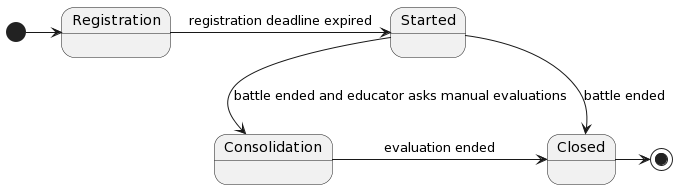
\includegraphics[width=1\textwidth]{Images/CKBLifecycle.png}
              \caption{Code kata battle lifecycle}
              \label{fig:CKBLifecycle}
        \end{figure}

    \item \textbf{Student Team Formation:} \\
    Upon entering a battle, a student has the capability to create a team by extending invitations to other students via email. The group initially resides in the Pending state until the commencement of the battle. At this point, if the team aligns with the specified requirements of the battle (the required number of students), the team's state transitions to Accepted. Contrarily, if the team falls short of meeting the stipulated requirements, the state shifts to Rejected.
    
        \begin{figure}[h!]
              \centering
              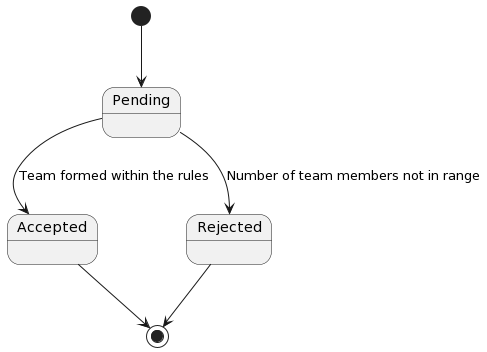
\includegraphics[width=0.7\textwidth]{Images/TeamFormation.png}
              \caption{Students team formation}
              \label{fig:CKBLifecycle}
        \end{figure}

    \item \textbf{GitHub Integration:} \\
    Following the creation of the repository by the educator, denoting the RepositoryCreated state, students are required to fork the repository. Subsequently, they must set up the automated workflow using GitHub Actions, marking the transition to the WorkflowEstablished state. As the battle concludes, the state progresses to BattleClosed, meaning that no further pushes to the repository are permitted.
        \begin{figure}[h!]
              \centering
              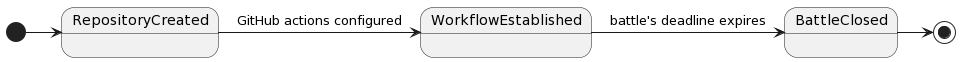
\includegraphics[width=1\textwidth]{Images/GitHubConfiguration.png}
              \caption{GitHub Integration}
              \label{fig:CKBLifecycle}
        \end{figure}
    

    \item \textbf{Battle Score Update:} \\
    At the onset of a battle and throughout its active phase (denoted by the Started state for the code kata battle), the battle score update operates in the RealTimeUpdate state. This signifies that with every push made by each student, the scores undergo real-time updates. Upon the expiration of the submission deadline, the state transitions to the ConsolidationStage. In this phase, the educator has the option to perform a manual evaluation of the students if desired. Following the manual evaluation or, if no manual evaluation is conducted, the state moves to the FinalScore, revealing the conclusive rank of the battle. This systematic flow ensures a seamless and structured progression throughout the different stages of the battle.
        \begin{figure}[h!]
              \centering
              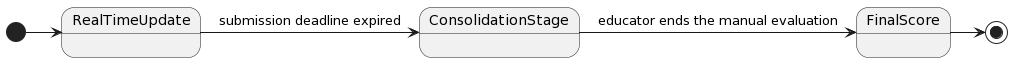
\includegraphics[width=1\textwidth]{Images/BattleScoreUpdate.png}
              \caption{Battle score update}
              \label{fig:CKBLifecycle}
        \end{figure}
    
\end{enumerate}

\subsection{Product functions}
\begin{enumerate}
    \item \textbf{Tournament Management} \\
    Only educators possess the authority to initiate the creation of a tournament on the CKB platform. Once a tournament concludes, the creator has the option to officially close it (only if all the battles are concluded). After the closure, the CKB platform signals the end of the competition notifying all participants. Throughout the tournament's progression, the educator can either personally add battles or delegate this task to other educators.

    \item \textbf{Code Kata Battle Management} \\
    The privilege of creating a Code Kata Battle within a tournament is reserved for educators. During this process, educators are asked to furnish essential details such as the kata description, the software project, build scripts, and scoring configurations, thereby shaping a well-defined coding challenge. In addition, educators have to establish timelines, including setting registration and submission deadlines for each battle. Furthermore, educators have the flexibility to determine the minimum and maximum number of individuals permitted within a team.

    \item \textbf{Student Interaction} \\
    Students have the option to register either individually for specific battles or collaboratively form teams, adhering to the predetermined team size limits. It's important to note that the team formation process occurs prior to the registration deadline.

    \item \textbf{GitHub Integration} \\
    Following the registration deadline, the platform generates a dedicated GitHub repository for each participating team, a repository that students are required to fork. Additionally, students must configure automated workflows utilizing GitHub Actions to facilitate continuous integration and evaluation. This setup ensures that with every commit made to the main branch, the CKB platform is triggered, updating scores in real time. This workflow guarantees efficient collaboration and real-time feedback for participating teams.

    \item \textbf{Scoring evaluation} \\
    The platform conducts automated evaluations encompassing functional aspects, timeliness, and source code quality. These evaluations result in real-time updates to scores, providing instant visibility for students and educators on the platform. Moreover, educators can perform manual evaluations and assign personal scores if necessary, contributing to a comprehensive and dynamic assessment process.
    
    \item \textbf{Gamification Badges} \\
    Educators can craft gamification badges tailored to specific tournaments, with each badge automatically assigned to students based on predefined rules and their performance. The earned badges become prominently displayed in a user's profile, offering a visual representation of their achievements. Both students and educators can access and view these badges, fostering a sense of recognition and accomplishment within the CKB platform.    

    \item \textbf{Notification System} \\
    The CKB platform ensures communication by automatically notifying students and educators of new tournaments, battles, and tournament closures. These notifications are comprehensive, offering essential information such as important deadlines and updates. This proactive approach improves user engagement and keeps participants well informed throughout their CodeKataBattle experience.
    
\end{enumerate}


\subsection{User characteristics}

\begin{enumerate}
    \item \textbf{Educators} \\
    An educator is a user with the power of managing the CKB platform. They have the authority to create, manage, and close tournaments. In addition, they can define code kata battles, and badges, and evaluate students' submissions.

    \item \textbf{Students} \\
     Students are the primary users who participate in code kata battles and tournaments. They register for battles, form teams, and actively engage in coding exercises.
        
\end{enumerate}

\subsection {Assumptions, dependencies and constraints}

\subsubsection{Assumptions}
The following assumptions are made to clarify the domain in which the software runs. Such assumptions are properties of CKB or conditions that the system takes for granted because they are out of its control. For that reason, they need to be verified to ensure the correct behavior of CKB.

\begin{table}[h]
    \centering
    \begin{tabular}{|l|l|}
    \hline
        D1 & The users (educators and students) have basic proficiency in using web-based platforms \\
        & and are familiar with version control systems, such as Git\\
    \hline
        D2 & Educators have the necessary knowledge to create meaningful code kata battles,\\ 
        & including defining test cases and scoring criteria \\
    \hline
        D3 & Educators and students can connect to the Internet with their devices \\
    \hline
        D4 & Notification must arrive to connected users in one minute \\
    \hline
        D5 & GitHub Account Requirement: students are required to have a GitHub account \\
        & for participation, and the platform assumes that students have the necessary permissions 
        \\ & to fork repositories \\
    \hline
        D6 & E-mail required \\
    \hline
        D7 & Users need a reliable internet connection to interact with the CKB platform\\
    \hline
    \end{tabular}
    \caption{Assumptions}
    \label{tab:assumptions}
\end{table}


\subsubsection{Dependencies}
In the previous sections, a number of dependencies from third-party software regarding core features of the systems has been identified:

\begin{table}[h]
    \centering
    \begin{tabular}{|l|l|}
    \hline
        DP1 & The CKB platform relies on GitHub for repository hosting and continuous\\
        &integration processes\\
    \hline
        DP2 & To allow static code analysis external API could be required\\
    \hline
    \end{tabular}
    \caption{Assumptions}
    \label{tab:assumptions}
\end{table}


\subsubsection{Constraints}
Since users will use the platform to compete and improve their coding skills the CKB platform must support a variety of programming languages.
In order to give a good user experience the CKB platform is optimized for modern web browsers (Chrome, Firefox, Safari) to allow each person to play with his favorite browser.
The platform must be designed to handle a scalable number of concurrent users during peak periods, such as registration deadlines. In addition, the platform must adhere to security best practices to protect user data and prevent unauthorized access, to prevent any malicious scripts from breaking into the system it exploits a sandboxing system to.